\chapter{Modelo de maturidade no processo}

Modelo de maturidade consiste em uma série de indicadores de qualidades de processo , fornecendo tal indicação em nível de maturidade. \cite{pressman}. Para \citeonline{pressman}, “sua finalidade é proporcionar uma indicação geral da “maturidade do processo” exibida por uma organização de software”.

Para as avaliações de processos de software existem dois modelos CMMI e o MPS.BR. “O CMMI ® (Capability Maturity Model ® Integration – Modelo Integrado de Maturidade e de Capacidade) é um modelo de maturidade para melhoria de processo, destinado ao desenvolvimento de produtos e serviços, e composto pelas melhores práticas associadas a atividades de desenvolvimento e de manutenção que cobrem o ciclo de vida do produto desde a concepção até a entrega e manutenção.” \cite{cmmi}

O MPS.BR é um programa que visa a Melhoria de Processos de Software e Serviços em duas metas: meta técnica e meta de negócio. A meta técnica está relacionada com a melhoria do modelo MPS, e meta de negócio consiste na difusão do modelo para auxiliar pequenas, médias (foco) e grandes organizações. \cite{mps}

Para esse trabalho foi estabelecido o uso do CMMI, por possuir suas práticas mais detalhadas.Assim, nesse capítulo
é apresentado um mapeamento das práticas do CMMI que estão relacionadas com as atividades do processo 
de Engenharia de Requisitos definido. Essas práticas são provenientes do nível 2 do CMMI com o processo
de Gerência de Requisitos e do nível 3 do CMMI com o processo de Desenvolvimento de Requisitos. Esse mapeamento pode
ser visto nas Figuras \ref{fig:gerencia} e \ref{fig:desenvolvimento}.

\section{Gerência de Requisitos}

Os objetivos das práticas escritas nessa seção foram baseadas nas descrições contidas no CMMI for Development publicado pela \citeonline{cmmi}.

\begin{figure}[!htb]
\centering
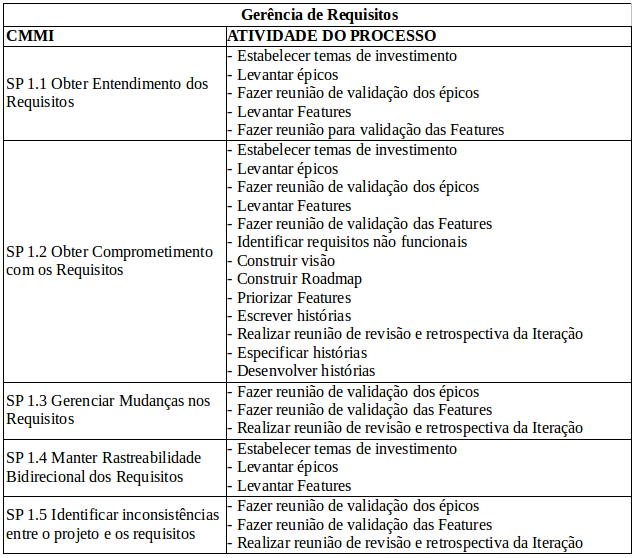
\includegraphics[scale=0.6]{figuras/gerencia.png}
\caption{Atividades do Processo com a Gerência de Requisitos do CMMI}
\label{fig:gerencia}
\end{figure}


Na prática específica de \textbf{Entender os Requisitos} estão envolvidas as atividades 
que permitem um entendimento dos requisitos através das técnicas de elicitação 
definidas para a familiarização com o processo, tais como: 
Estabelecer tema de investimento, Levantar épicos, Levantar \textit{Features}. Além disso,
o entendimento dos requisitos pode ser obtido através de reuniões de validação com o 
cliente, atividades essas nomeadas como: Fazer reunião de validação dos épicos e fazer 
reunião de validação das \textit{features}.

Na prática específica de \textbf{Obter Compromisso para os requisitos}, a medida que os 
requisitos evoluem, esta prática garante que ao longo do projeto seja obtido um 
comprometimento para com os requisitos em todas as suas fases. No processo definido 
neste trabalho desde a primeira atividade que envolvem os requisitos até aquelas que 
tratam deles em suas últimas fases, os requisitos têm a sua devida atenção para que o 
projeto seja desenvolvido com qualidade. 

Durante o processo definido neste trabalho, os requisitos podem sofrer alterações por 
diversos motivos. Nesta prática específica, \textbf{Gerenciar mudanças de requisitos}, a
medida que há mudanças no projeto, estas devem ser documentadas e devem ficar claras para
todos os envolvidos para que não ocorram inconsistências ao decorrer do projeto. 
Por isso, a prática de gerenciar mudanças nos requisitos envolvem as seguintes atividades de 
validação: Fazer reunião de validação dos épicos, Fazer reunião de validação das 
\textit{features} e Realizar reunião de revisão e retrospectiva de Iteração), 
pois são nelas que obtém-se validação das atividades realizadas e, caso ocorram 
mudanças, serão nelas que estas mudanças serão documentadas e esclarecidas. 

Quando há um bom gerenciamento dos requisitos, a sua rastreabilidade dos requisitos é 
gerenciada desde a sua origem até a sua última fase de detalhamento. Na prática específica
de \textbf{Manter a rastreabilidade bidirecional dos requisitos}, tarefas específicas das
atividades, tais como relacionar épicos ao tema de investimento, relacionar 
\textit{features} aos épicos e relacionar histórias às \textit{features}, esta
rastreabilidade será garantida para que seja obtida a origem dos requisitos.

Na prática específica de \textbf{Identificar inconsistências entre o projeto e os 
requisitos}, deve-se procurar inconsistências no projeto em todos os seus processos e 
corrigí-las. Esta prática se encontra nas atividades de validação dos requisitos tais
como, Fazer reunião de validação dos épicos, Fazer reunião de validação das 
\textit{features} e Realizar reunião de revisão e retrospectiva da iteração, pois são 
nas validações que essas inconsistências serão identificadas e corrigidas.

\section{Desenvolvimento de Requisitos}

Os objetivos das práticas escritas nessa seção foram baseadas nas descrições contidas no CMMI for Development publicado pela \citeonline{cmmi}.

\begin{figure}[!htb]
\centering
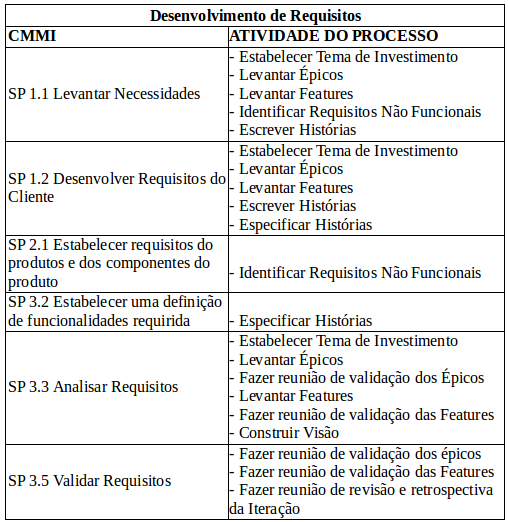
\includegraphics[scale=0.6]{figuras/desenvolvimento.png}
\caption{Atividades do Processo com o Desenvolvimento de Requisitos do CMMI}
\label{fig:desenvolvimento}
\end{figure}

Na prática específica \textbf{Levantar necessidades} as expectativas e necessidades dos usuários
são identificadas. Nas atividades Estabelecer Tema de Investimento, Levantar Épicos, 
Levantar \textit{Features}, Identificar Requisitos Não Funcionais e Escrever Histórias ocorre 
essa identificação por meio das técnicas de elicitação definidas na seção \ref{tecnicas}, que são: Análise
Documental, \textit{Workshop} de Requisitos e Entrevistas.

Na prática específica \textbf{Desenvolver Requisitos de Cliente} as necessidades levantadas são
convertidas em requisitos documentados, denominados Requisitos de Cliente. Nas atividades Estabelecer Tema de Investimento, Levantar Épicos, 
Levantar \textit{Features}, Escrever Histórias e Especificar Histórias ocorre 
a especificação dos requisitos levantados. A atividade de Especificar Histórias
atende bem à essa prática, pois é a especificação das histórias levantadas na atividade
de Escrever Histórias e também contém os critérios de aceitação que atende a subprática
de definir estratégia de verificação e validação.

Na prática específica \textbf{Estabelecer uma Definição da Funcionalidade Requerida}
o objetivo é analisar as funcionalidades para identificar ações, sequências, entradas e saídas.
Na atividade Especificar histórias essa prática é atendida pois há a especificação
das histórias e a escrita dos testes de aceitação que proporcionam essa visão das ações,
entradas e saídas nas funcionalidades.

Na prática específica \textbf{Analisar Requisitos} o objetivo é analisar os requisitos
para determinar se estão alinhados com os requisitos de mais alto nível, se estão de acordo
com o que o cliente estabeleceu. Nas atividades Fazer reunião de validação dos Épicos,
Fazer reunião de validação dos \textit{Features} e Realizar Reunião de Revisão e Retrospectiva da Iteração
os requisitos levantadas e especificados são validados para confirmar se atendem às necessidades
dos clientes. 

Na prática específica \textbf{Validar Requisitos} o objetivo é garantir que os requisitos 
identificados e documentados estejam de acordo com o requerido. Nas atividades Fazer reunião de validação dos Épicos,
Fazer reunião de validação dos \textit{Features} e Realizar Reunião de Revisão e Retrospectiva da Iteração
essa prática é atendida, pois se tratam de reuniões para validações dos requisitos
nos diferentes graus de abstração. Todavia, na Reunião de Revisão e Retrospectiva da Iteração
a validação é feita na implementação dos requisitos.